% !TeX root = thesis.tex
% !TeX spellcheck = en_US
% !TeX encoding = UTF-8
%\documentclass[]{report}
\documentclass[english, LaM, oneside]{sapthesis}%remove "english" for a thesis written in Italian

%\usepackage[utf8]{inputenx}
%\usepackage{xcolor}
%\usepackage{indentfirst}
%\usepackage{microtype}

%\usepackage{lettrine}
\linespread{0.9}

% This can be used to make space between section names more compact. The titlesec package allows changing how chapters are displayed, numerated, etc.
%\usepackage[compact]{titlesec}
% to get the bibliography in the toc
\usepackage[nottoc,notlot,notlof,chapter]{tocbibind}

\newcommand{\thesistitle}{Reward shaping in RL for {\sc LTL}$_f$/{\sc LDL}$_f$ Goals: Theory and Practice}

\usepackage{index}
\usepackage{hyperref}
\usepackage{wrapfig}
\usepackage[round]{natbib}
\bibliographystyle{plainnat}

\usepackage[intoc,refpage]{nomencl} %refeq
\makenomenclature

%\usepackage{qtree}
% The algorithm packages have to be after hyperref.
\usepackage{algorithm, algorithmic} %algpseudocode
\usepackage{mathtools}
\usepackage{amssymb, amsmath}
\usepackage{xspace, float, graphicx, pstricks}
%\usepackage[autostyle]{csquotes}  
\usepackage{graphicx}
\graphicspath{{./images/}}


\hypersetup{
	hyperfootnotes=true,            
	bookmarks=true,         
	colorlinks=true,
	linkcolor=red,
	linktoc=page,
	anchorcolor=black,
	citecolor=red,
	urlcolor=blue,
	pdftitle={\thesistitle},
	pdfsubject = {Master Thesis, University of Rome "La Sapienza"},
	pdfauthor={Marco Favortio},
	pdfkeywords={thesis, sapienza, roma, university}
	pdfauthor = {\textcopyright\ \today\ Marco Favorito},
}



%opening
\title{\thesistitle}
\author{Marrco Favorito}
\IDnumber{1609890}
\course[]{Master in Engineering in Computer Science}
\courseorganizer{Facolt\`a di Ingegneria dell'Informazione, Informatica e Statistica}
\submitdate{2017/2018}
\copyyear{2018}
\advisor{Prof. Giuseppe De Giacomo}
\coadvisor{Dr. co-advisor}
\authoremail{favorito.1609890@studenti.uniroma1.it}
\examdate{1}
\examiner{Prof. ...} \examiner{Prof. ...} \examiner{Prof. ...}  \examiner{Prof. ...}  \examiner{Prof. ...} \examiner{Prof. ...}  \examiner{Prof. ...} 




\begin{document}
	%%%%%%%%%%%%%%%%%%%%%%%%%% General

\newcommand{\myi}{(\emph{i})\xspace}
\newcommand{\myii}{(\emph{ii})\xspace}
\newcommand{\myiii}{(\emph{iii})\xspace}
\newcommand{\myiv}{(\emph{iv})\xspace}
\newcommand{\myv}{(\emph{v})\xspace}
\newcommand{\myvi}{(\emph{vi})\xspace}
\newcommand{\myvii}{(\emph{vii})\xspace}
\newcommand{\myviii}{(\emph{viii})\xspace}

%% general math
%\newcommand{\A}{\mathcal{A}} 
\newcommand{\B}{\mathcal{B}}
%\newcommand{\C}{\mathcal{C}} 
\newcommand{\D}{\mathcal{D}}
\newcommand{\E}{\mathcal{E}} \newcommand{\F}{\mathcal{F}}
\newcommand{\G}{\mathcal{G}} \renewcommand{\H}{\mathcal{H}}
\newcommand{\I}{\mathcal{I}} \newcommand{\J}{\mathcal{J}}
\newcommand{\K}{\mathcal{K}} \renewcommand{\L}{\mathcal{L}}
\newcommand{\M}{\mathcal{M}} \newcommand{\N}{\mathcal{N}}
\renewcommand{\O}{\mathcal{O}} \renewcommand{\P}{\mathcal{P}}
\newcommand{\Q}{\mathcal{Q}} \newcommand{\R}{\mathcal{R}}
\renewcommand{\S}{\mathcal{S}} \newcommand{\T}{\mathcal{T}}
\newcommand{\U}{\mathcal{U}} \newcommand{\V}{\mathcal{V}}
\newcommand{\W}{\mathcal{W}} \newcommand{\X}{\mathcal{X}}
\newcommand{\Y}{\mathcal{Y}} \newcommand{\Z}{\mathcal{Z}}

\newcommand{\limp}{\mathbin{\rightarrow}}
\newcommand{\ind}{\hspace*{.18in}}

%% LTL
\newcommand{\Next}{\raisebox{-0.27ex}{\LARGE$\circ$}}
\newcommand{\Wnext}{\raisebox{-0.27ex}{\LARGE$\bullet$}}
\newcommand{\Until}{\mathop{\U}}
\newcommand{\Since}{\mathop{\S}}
\newcommand{\Release}{\mathop{\R}}
\newcommand{\Wuntil}{\mathop{\W}}
\newcommand{\true}{\mathit{true}}
\newcommand{\final}{\mathit{Final}}
\newcommand{\false}{\mathit{false}}
\newcommand{\ttrue}{{\mathit{tt}}}
\newcommand{\ffalse}{\mathit{ff}}
\newcommand{\Last}{\mathit{last}}
\newcommand{\Ended}{\mathit{end}}
\newcommand{\length}{\mathit{length}}
\newcommand{\last}{\mathit{n}}
\newcommand{\nnf}{\mathit{nnf}}
\newcommand{\BOX}[1]{ [#1]}
\newcommand{\DIAM}[1]{\langle #1 \rangle}
\newcommand{\transl}{f}


%% Logics
\newcommand{\FOL}{{\sc fol}\xspace}
\newcommand{\LT}{{\sc lt}$_f$\xspace}
\newcommand{\LTi}{{\sc lt}$_i$\xspace}
\newcommand{\LTL}{{\sc ltl}\xspace}
\newcommand{\LTLf}{{\sc ltl}$_f$\xspace}
\newcommand{\LDL}{{\sc ldl}\xspace}
\newcommand{\LDLf}{{\sc ldl}$_f$\xspace}
\newcommand{\RE}{{\sc re}$_f$\xspace}
\newcommand{\REGEX}{{\sc re}\xspace}
\newcommand{\PDL}{{\sc pdl}\xspace}
\newcommand{\FOf}{{\sc fo}$_f$\xspace}
\newcommand{\MSOf}{{\sc mso}$_f$\xspace}
\newcommand{\FO}{{\sc fo}\xspace}
\newcommand{\MSO}{{\sc mso}\xspace}
%\newcommand{\ATA}{{\sc ata}\xspace}
\newcommand{\AFW}{{\sc afw}\xspace}
\newcommand{\NFA}{{\sc nfa}\xspace}
\newcommand{\DFA}{{\sc dfa}\xspace}
\newcommand{\DFAs}{{\sc dfa}s\xspace}
\newcommand{\declare}{{\sc declare}\xspace}
\newcommand{\fol}{\mathit{fol}}
\newcommand{\f}{\mathit{f}}
%\newcommand{\g}{\mathit{g}}
\newcommand{\re}{\mathit{re}}


\newcommand{\tup}[1]{\langle #1 \rangle}

\newcommand{\Stop}{\mathit{stop}}
\newcommand{\rew}{\mathit{rew}}
\newcommand{\Tr}{\mathit{Tr}}

\newcommand{\LOGSPACE}{{\sc logspace}\xspace}
\newcommand{\NLOGSPACE}{{\sc nlogspace}\xspace}
\newcommand{\PTIME}{{\sc ptime}\xspace}
\newcommand{\NP}{{\sc np}\xspace}
\newcommand{\EXPTIME}{{\sc exptime}\xspace}
\newcommand{\PSPACE}{{\sc pspace}\xspace}
\newcommand{\TWOEXPTIME}{{\sc 2exptime}\xspace}


\newcommand{\expand}{\textbf{\textit{E}}}
\newcommand{\ttt}{{\textbf{\textit{T}}}}
\newcommand{\fff}{{\textbf{\textit{\texttt{F}}}}}

\newcommand{\fstate}{s_f}

\newcommand{\atomize}[1]{\texttt{"}\ensuremath{#1}\texttt{"}}


% misc


%RL
\newcommand{\MDP}{\M}
\newcommand{\States}{S}
\newcommand{\Actions}{A}
\newcommand{\TrFun}{T}
\newcommand{\Reward}{R}
\newcommand{\DiscFact}{\gamma}
\newcommand{\Policy}{\rho}
\newcommand{\ExpRet}{G}
\newcommand{\ValFun}{v}
\newcommand{\qFun}{q}

\newcommand{\ValOptFun}{\ValFun^*}
\newcommand{\qOptFun}{\qFun^*}
\newcommand{\OptPolicy}{\Policy^*}

\newcommand{\ValFunEst}{V}
\newcommand{\qFunEst}{Q}
\newcommand{\LRate}{\alpha}

\newcommand{\NMRDP}{\N}
\newcommand{\NMReward}{\bar{\Reward}}
\newcommand{\NMPolicy}{\bar{\Policy}}

%LOGIC

\newcommand{\Prop}{\P}
\newcommand{\PropInt}{\Pi}
\newcommand{\PropFormula}{\phi}
\newcommand{\trace}{\pi}
\newcommand{\Kripke}{\K}
\newcommand{\tm}[1]{\ \text{#1}\ }
\newcommand{\tiff}{\tm{iff}}

\newcommand{\automaton}{\mathcal{A}}
\newcommand{\LLf}{\LTLf/\LDLf}
\newcommand{\DfunSym}{\partial}
\newcommand{\Dfun}[1]{\DfunSym\lparen #1,\PropInt \rparen}
\newcommand{\AND}{\wedge}
\newcommand{\OR}{\vee}
\newcommand{\NOT}{\lnot}
\newcommand{\regexp}{\varrho}
\newcommand{\TrueDelta}[1]{\textit{\textbf{\texttt{T}}}_{#1}}
\newcommand{\FalseDelta}[1]{\textit{\textbf{\texttt{F}}}_{#1}}


\newcommand{\Sapientino}{{\sc sapientino}\xspace}
\newcommand{\Breakout}{{\sc breakout}\xspace}
\newcommand{\Minecraft}{{\sc minecraft}\xspace}

%math

\newcommand{\set}[1]{\{#1\}}
\newcommand{\Naturals}{\mathbb{N}}
\newcommand{\Reals}{\mathbb{R}}
\newcommand{\defeq}{\coloneqq}



%%% Local Variables:
%%% mode: latex
%%% TeX-master: "main"
%%% save-place: t
%%% End:

	
	\frontmatter	
	\maketitle
	
	\begin{abstract}
		write your abstract here
	\end{abstract}
	
	\tableofcontents
	
	\mainmatter
	\chapter{Introduction}
This chapter presents the outline of this thesis and summarizes motivations, goals, and achievements.

\section{Reinforcement Learning}
Reinforcement learning is an area of Machine Learning where the learning comes from rewards and punishments \citep{Sutton:1998:IRL:551283}. It is concerned in how the learning entity, the \emph{agent}, interacting in an \emph{environment}, should take \emph{actions} so to maximize the observed \emph{reward}. The reward signal is observed after each action taken by the agent. The agent chooses actions depending on the current state of the environment. A solution to the reinforcement learning problem is a \emph{policy} which determines which action should
be executed in a given state in order to maximize the long term reward. An algorithm that tackles this kind of problem is called \emph{reinforcement learning algorithm}.

\medskip
The problem, due to its generality, is studied in many other disciplines, such as \emph{game theory}, \emph{control theory}, \emph{operations research}, \emph{multi-agent system}, and many others. Usually, in order to simplify the tractability of the problem, it is assumed that the environment can be modeled as a \emph{Markov Decision Process} (MDP). An environment behaves like an MDP if the Markov property is satified, which means that the state space representation in the algorithm captures enough details so that the optimal decisions can be made when the information about only the current state is available. 

\medskip
Even if the laws that determines the evolution of the systems and the rewards are unknown a priori, it is still possible to solve an MDP by making several simulations and gathering experiences about the visited states, the actions taken and the observed rewards. However, many challenges arise in this settings:
\begin{itemize}
	\item \emph{Exponential state space explosion}: due to the feature selection used for the state space encoding, every added feature yields exponential increase in the number of states, hence reducing the tractability of the problem.
	\item \emph{Exploration-Exploitation trade-off}: due to the former issue, reinforcement learning algorithm should be designed to avoid exploring irrelevant states in terms of expected reward, while preferring the ones with high expected reward (\emph{exploitation}). Furthermore, the algorithms should be sensitive to the local optima issue, a well-known in statistical learning literature (\emph{exploration}).
	\item \emph{Temporal credit assignment}: the agent should be able to foresee the effect of his actions (in terms of expected reward), due to the fact that, in many domains, the current reward is influenced by past decisions.
\end{itemize}

This problems lead to the use of heuristics and approximate solutions. A simple way to do reinforcement learning is to use exploration which is based on the current policy with a certain degree of randomness which deviates from such a policy.

\section{Rewarding behaviors}
In some domains it could be of interest the study of rewards not depending on a single decision (like in MDPs) but depending on a \emph{sequence} of visited states and actions. For instance, we can reward an agent not only by reaching a goal state, but if the goal is reached while satisfying other properties of interest during the simulation or, in other words, if the agent satisfies some target behavior. It is clear that the the definition of MDP does not fit this problem, since the optimal decision in the current state depends from the \emph{history of states} that leads to the current state.

\medskip

This idea of rewarding behaviors has been proposed in \citep{bacchus1996rewarding}, by defining the \emph{Non-Markovian Reward Decision Process} (NMRDP), a variant of an MDP where the reward does not depend only from one transition of the environment but from a sequence of transitions. In order to specify the desired behaviors that the agent should learn, they defined a temporal logic formalisms called \PLTL (Past \LTL), which is able to speak about a sequence of property configurations over time, that we call \emph{traces}. The classic reinforcement learning algorithms does not work on an NMRDP; however, they propose a transformation from NMRDP into an \emph{expanded} MDP such that the solution of the MDP is also a solution of the original problem. Hence, in order to solve the NMRDP, we can run off-the-shelf RL algorithms over the transformed MDP; the learnt Markovian policy can be easily converted into an optimal policy for the NMRDP.

The trick here is that the transformed MDP is defined over an \emph{expanded state space}, which still contains the original state space but enriches it by labeling every state. The idea is that the labels should keep track in some way the (partial) satisfaction of the temporal formulas. As a result, every state in the transformed state space is replicated multiple times, marking the difference between different (relevant) histories terminating in that state.

\medskip
A similar transformation has been done in the following works: 
\citep{ThiebauxGSPK06} and \citep{gretton2014more}, where the temporal logic formalism was respectively \FLTL (a finite \LTL with future formulas) and \FstarLTL (a variant of \FLTL); 
in \citep{icarte2018teaching}, where they used \emph{Co-Safe} \LTL formulas \citep{Kupferman:2001:MCS:569028.569032, Lacerda:2015:OPG:2832415.2832470};
in \citep{CamachoCSM17, CamachoCSM17b}, where they used \LTLf (Linear Temporal Logic over finite traces) \citep{de2013linear}.
In \citep{AAAI1817342} the specification of temporal goals is done by \LTLf or \LDLf (Linear Dynamic Logic over finite traces) formulas.

\section{Topic of the Thesis}\label{sect:topic-thesis}
In this thesis, we leverage the construction of \citep{AAAI1817342} to define a new problem. Consider a classic reinforcement learning problem defined by an MDP. The agent acts in the state space of the MDP and tries to maximize the reward. We can think of the features of this state space as \emph{low-level features}, e.g. the coordinates of a robot in a room, informations about the limbs etc. 

Now consider that we want to talk about some high-level properties of the environment, e.g. continuing with the example of the robot in the room, we are interested in the status of the window and the door (if they are open or closed). We can define the fluents $open\_window$ and $open\_door$, respectively. We call the features to determine the status of the fluents \emph{high-level features}.

Given this setting, we are interested in:
\begin{itemize}
	\item maximize the reward of the original MDP;
	\item maximize the reward specified by temporal formulas, expressed in \LLf, over the fluents 
\end{itemize}
E.g. in the example, a temporal specification could be "eventually open the window, then eventually open the door". 

In this work we specify formally the just defined problem, propose the transformation into an MDP and prove the equivalence of the transformation with the original problem. We propose also a way to apply reward shaping techniques to improve the learning in terms of convergence rate. Moreover, we provide an implementation and give experimental evidence of the goodness of our construction.

\section{Structure of the Thesis}
The rest of the thesis is structured as follows:
\begin{itemize}
	\item In Chapter \ref{ch:logic} we describe the notions about temporal logic formalisms, that will be used for temporal goal specifications. We start from \LTL, \REGEX and then we move towards \LTLf and \LDLf, upon which our method is built on.
	\item In Chapter \ref{ch:flloat} we describe FLLOAT, a software project that implements the translation from \LLf formulas to equivalent automata. Such translation is an important piece of our approach;
	\item Chapter \ref{ch:rl} is the core of the thesis. We introduce foundational concepts in reinforcement learning, MDPs and algorithm to find a solution. Then we move to NMRDPs and we formally describe our approach.
	\item In Chapter \ref{ch:reward-shaping} we apply reward shaping techniques to the setting explained in Chapter \ref{ch:rl}.
	\item In Chapter \ref{ch:rltg} we present a reinforcement learning framework allowing easy implementation of the construction described in Chapter \ref{ch:rl} and \ref{ch:reward-shaping}.
	\item Chapter \ref{ch:experiments} describes the conducted experiments,5 giving evidence that our approach actually works.
	\item The thesis is concluded in Chapter \ref{ch:conclusions}. This chapter summarizes also the achievements of
	the thesis and discusses future work.
\end{itemize}

	\chapter{Preliminaries}
\label{preliminaries}
In this chapter we describe the background knowledge required for this work. We introduce Markov Decision Process (MDP) and Non-Markovian Reward Decision Process (NMRDP), common formalisms in the context of Reinforcement Learning. We describe Linear Temporal Logic over finite traces (\LTLf) and Linear Dynamic Logic over finite traces (\LDLf), that we use for define temporal goal in a RL setting. Then, we describe an important result about RL for NMRDP with \LTLf/\LDLf rewards, that is the basis for this work.

\section{Reinforcement Learning}
\label{RL}
Reinforcement Learning \citep{Sutton:1998:IRL:551283} is a sort of optimization problem where an \emph{agent} interacts with an \emph{environment} and obtains a \emph{reward} for each action he chooses and the new observed state. The task is to maximize a numerical reward signal obtained after each action during the interaction with the environment. The agent does not know a priori how the environment works (i.e. the effects of his actions), but he can make observations in order to know the new state and the reward. Hence, learning is made in a \emph{trial-and-error} fashion. Moreover, it is worth to notice that in many situation reward might not been affected only from the last action but from an indefinite number of previous action. In other words, the reward can be \emph{delayed}, i.e. the agent should be able to foresee the effect of his actions in terms of future expected reward. 

In the next subsections we introduce some of the classical mathematical frameworks for RL: Markov Decision Process (MDP) and Non-Markovian Reward Decision Process (NMRDP).
\subsection{Markov Decision Process}
\label{MDP}

	A Markov Decision Process (MDP) $\MDP$ is a tuple $\tup{\States, \Actions, \TrFun, \Reward, \DiscFact}$ containing a set of \emph{states} $\States$, a set of \emph{actions} $\Actions$, a \emph{transition function} $\TrFun: \States \times \Actions \to Prob(\States)$ that returns for every pair state-action a probability distribution over the states, a \emph{reward function} $\Reward: \States \times \Actions \times \States \to \Reals$ that returns the reward received by the agent when he performs action $a$ in $s$ and transitions in $s'$, and a \emph{discount factor} $\DiscFact$, with $0 \le \DiscFact \le 1$, that indicates the present value of future rewards.
	
	A \emph{policy} $\Policy: \States \to \Actions$ for an MDP $\MDP$ is a mapping from states to actions, and represents a solution for $\MDP$. Given a sequence of rewards $\Reward_{t+1}, \Reward_{t+2}, \dots, \Reward_{T}$, the \emph{expected return} $\ExpRet_t$ at time step $t$
	is defined as: 
	\begin{equation}
		\ExpRet_t \defeq \sum_{t=k+1}^T \DiscFact^{k-t-1}\Reward_k
	\end{equation} where can be $T = \infty$ and $\DiscFact = 1$ (but not both). 
	
	The \emph{value function} of a state $s$, the \emph{state-value function} $\ValFun_\Policy(s)$ is defined as the expected return when starting in $s$ and following policy $\Policy$, i.e.:
	\begin{equation}
	\label{state-value-fun}
		\ValFun_\Policy(s) \defeq \mathbb{E}_{\Policy}[\ExpRet_t | \States_t = s], \forall s \in \States
	\end{equation}
	
	Similarly, we define $\qFun_\Policy$, the \emph{action-value function for policy $\Policy$}, as:
	\begin{equation}
		\label{action-value-fun}
		\qFun_\Policy(s, a) \defeq \mathbb{E}_{\Policy}[\ExpRet_t | \States_t = s, \Actions_t = a], , \forall s \in \States, \forall a \in \Actions
	\end{equation}
	
	Notice that we can rewrite \ref{state-value-fun} and \ref{action-value-fun} recursively, yielding the \emph{Bellman equations}:
	
	\begin{equation}
	\label{bellman-state-value-fun}
	\ValFun_\Policy(s) =  \sum_{s'} P(s' | s,a)[\Reward(s,a,s') + \DiscFact \ValFun(s')] 
	\end{equation}
	
	where we used the definition of the transition function:
	\begin{equation}
	\TrFun(s,a,s') = P(s' | s,a)
	\end{equation}
	
	We define the \emph{optimal state-value function} and the \emph{optimal action-value function} as follows:
	\begin{equation}
	\label{optimal-state-value-fun}
		\ValOptFun(s)  \defeq \max_\Policy  \ValFun_\Policy(s), \forall s\in \States		
	\end{equation}
	
	\begin{equation}
	\label{optimal-action-value-fun}
	\qOptFun(s, a) \defeq \max_\Policy  \qFun_\Policy(s, a), \forall s\in \States, \forall a\in \Actions
	\end{equation}
	
	Notice that with \ref{optimal-state-value-fun} and \ref{optimal-action-value-fun} we can show the correlation between $\ValOptFun_\Policy(s)$ and $\qOptFun_\Policy(s, a)$:
	
	\begin{equation}
		\qOptFun(s, a) = \mathbb{E}_\Policy[R_{t+1} + \DiscFact \ValOptFun_\Policy(\States_{t+1})| \States_t = s, \Actions_t = a]
	\end{equation}
	
	
	We can define a partial order over policies using value functions, i.e. $\forall s\in \States. \Policy \ge \Policy' \iff \ValFun_\Policy(s) \ge \ValFun_{\Policy'}(s)$. An \emph{optimal policy} $\OptPolicy$ is a policy such that $\OptPolicy \ge \Policy$ for all $\Policy$. 
	
	
\subsection{Temporal Difference Learning}

\emph{Temporal difference learning} (TD) refers to a class of model-free reinforcement learning methods which learn by bootstrapping from the current estimate of the value function. These methods sample from the environment, like Monte Carlo (MC) methods, and perform updates based on current estimates, like dynamic programming methods (DP). We do not discuss MC and DP methods here.

Q-Learning and Sarsa are such a methods. They updates $\qFunEst(s, a)$, i.e. the estimation of $\qOptFun(s, a)$ at each transition $(s, a) \to (s', r)$. Q-Learning uses the following update rule:
\begin{equation}
\qFunEst(s, a) \leftarrow \qFunEst(s, a) + \LRate [r + \DiscFact \max_{a'} \qFunEst(s', a') - \qFunEst(s, a)]
\end{equation}

while Sarsa:
\begin{equation}
\qFunEst(s, a) \leftarrow \qFunEst(s, a) + \LRate [r + \DiscFact \qFunEst(s', a') - \qFunEst(s, a)]
\end{equation}

TD$(\lambda)$ is an algorithm which uses \emph{eligibility traces}. The parameter $\lambda$ refers to the use of an eligibility trace. The algorithm generalizes MC methods and TD learning, obtained respectively by setting $\lambda = 1$ and $\lambda = 0$. Intermediate values of $\lambda$ yield methods that are often better of the extreme methods. Q-Learning and Sarsa that has been shown before can be rephrased with this new formalism as Q-Learning(0) and Sarsa(0), special cases of Watkin's Q$(\lambda)$ and Sarsa($\lambda$).

\section{\LTLf and \LDLf}
In this section we introduce \LTLf and \LDLf, two formalisms that we will use for define the reward function of a RL task over \emph{sequence of transitions} rather than one transition.

\subsection{Linear Temporal Logic on Finite Traces: \LTLf}
Linear-time Temporal Logic over finite traces, \LTLf, is essentially standard 
\LTL \citep{Pnueli:1977:TLP:1382431.1382534} interpreted over finite, instead of over infinite, traces \citep{de2013linear}.

Indeed, the syntax of \LTLf is the same of \LTLf, i.e. \emph{formulas} of \LTLf are built from a set $\Prop$ of propositional symbols and are closed under the boolean connectives, the unary temporal operator \Next (\emph{next-time}) and the binary operator $\Until$ (\emph{until}):

\[\begin{array}{rcl}
\varphi &::=& \phi \mid \lnot \varphi \mid \varphi_1\land \varphi_2 \mid \Next\varphi \mid \varphi_1 \Until \varphi_2
\end{array}
\]
With $A\in \Prop$.

We use the standard abbreviations:
$\varphi_1\lor\varphi_2 \doteq \lnot(\lnot \varphi_1\land \lnot
\varphi_2)$;
\emph{eventually} as $\Diamond\varphi \doteq \true\Until\varphi$;
\emph{always} as $\Box\varphi \doteq\lnot\Diamond\lnot\varphi$; 
week next $\Wnext\varphi \doteq \lnot\Next\lnot\varphi$ (note that on finite
traces $\lnot\Next\varphi \not\equiv \Next\lnot\varphi$); and $Last \doteq \Wnext\false$ denoting the end of the trace. 

Formally, a \emph{finite trace} $\pi$ is a finite word over the alphabet $2^\Prop$, i.e. as alphabet we have all the possible propositional interpretations of the propositional symbols in $\Prop$. For the semantics we refer to \citep{de2013linear}.

\LTLf is as expressive as 
first-order logic (\FO)
over finite traces
and star-free regular expressions (\REGEX).

\subsection{Linear Dynamic Logic on Finite Traces: \LDLf}
\LDLf, \emph{Linear Dynamic Logic of Finite Traces} merges \LTLf with \REGEX$_f$ (\REGEX on finite traces) in a very natural way.
The logic is called LDL f
\LTLf can be extended to 


 which is expressive as monadic second-order logic 
(\MSO) over finite traces \cite{de2013linear}.

Linear Dynamic Logic of Finite
Traces

%Formally, \LDLf formulas $\varphi$ are built as follows:
%%%
%\[\begin{array}{lcl}
%\varphi &::=& \ttrue  \mid \lnot \varphi \mid \varphi_1 \land \varphi_2 \mid \DIAM{\varrho}\varphi \\
%\varrho &::=& \phi \mid \varphi? \mid  \varrho_1 + \varrho_2 \mid \varrho_1; \varrho_2 \mid \varrho^*
%\end{array}
%\]
%%%
%where $\ttrue$ stands for logical true; $\phi$ is a propositional
%formula over $\Prop$; $\varrho$ denotes path expressions, which are \REGEX over
%propositional formulas $\phi$ with the addition of the test construct
%$\varphi?$ typical of \PDL.  We use abbreviations
%$\BOX{\varrho}\varphi\doteq\lnot\DIAM{\varrho}{\lnot\varphi}$ as in \PDL.
%Intuitively, $\DIAM{\varrho}\varphi$ states that, from the current step
%in the trace, there exists an execution satisfying the \REGEX $\varrho$ 
%such that its last step satisfies $\varphi$, while
%$\BOX{\varrho}\varphi$ states that, from the current step, all executions
%satisfying the \REGEX $\varrho$ are such that their last step
%satisfies $\varphi$.
%%
%Tests are used to insert into the execution path checks for
%satisfaction of additional \LDLf formulas.
%
%
%%%
%Given an \LTLf/\LDLf formula $\varphi$,
%we can construct a deterministic finite state automaton (\DFA)~\cite{RaSc59} 
%$\A_\varphi$ that tracks satisfaction of $\varphi$, 
%given a finite trace~\footnote{An analogous
%	transformation to automata applies to several other formalisms for
%	representing non-Markovian rewards  \cite{BBG96,ThiebauxGSPK06,Slaney05,Gretton07,Gretton14,LacerdaPH14,LacerdaPH15}. 
%	All results presented here apply to those formalisms as well.},
%accepting a sequence of propositional interpretations {\em
%	iff} the sequence satisfies $\varphi$. This construction
%is a key element in the efficient transformation from non-Markovian
%rewards to Markovian rewards over an extended MDP \cite{BDP-AAAI18}.
%%%
%
%The idea is to use \LTLf/\LDLf formulas to specify when sequences of 
%state-action pairs, rather than one pair only, should be rewarded.
%Notice that we can easily incorporate the executed action in the current state
%by using propositions. In this way, we can make \LTLf/\LDLf deal with 
%actions, as well. From now on, we assume this is the case.

\newcommand{\Rnm}{\bar{R}}
\newcommand{\rhonm}{\bar{\rho}}





\subsection{\LTLf and \LDLf translation to automata}

\section{RL for NMRDP with \LTLf/\LDLf rewards}
In this section we introduce the formalism of Non-Markovian Reward Decision Process \citep{BacchusBG96} 
\subsection{Non-Markovian Reward Decision Process}
\label{NMRDP}
A Non-Markovian Reward Decision Process (NMRDP) $\NMRDP$ is a tuple $\tup{\States, \Actions, \TrFun, \NMReward, \DiscFact}$ where everything is defined as in the MDP but the reward function is defined as $\NMReward : (\States \times \Actions)^* \to \Reals$, i.e. is defined over sequences of states and actions. 	Given a trace $\pi = \tup{s_0, a_0, s_1, a_1, \dots, s_n, a_n}$, the \emph{value of $\pi$} is:
$$
v(\pi) = \sum_{i=1}^{|\pi|} \DiscFact^{i-1}\NMReward(\tup{\pi(1), \pi(2), \dots, \pi(i)})
$$
where $\pi(i) = (s_i, a_i)$.

The policy $\NMPolicy$ in this setting is defined over sequences of states, i.e. $\NMPolicy: \States^* \to \Actions$. 

The \emph{value of $\NMPolicy$} given an initial state $s_0$ is defined as:

$$
\ValFun^{\NMPolicy}(s) = \mathbb{E}_{\pi \sim \MDP, \NMPolicy, s_0}[v(\pi)]
$$
i.e. the expected value in state $s$ considering the distribution of traces defined by the transition function of $\MDP$, the policy $\NMPolicy$ and the initial state $s_0$.


	\chapter{RL for {\sc LTL}$_f$/{\sc LDL}$_f$ Goals}

\section{Reinforcement Learning}
\label{RL}
Reinforcement Learning \citep{Sutton:1998:IRL:551283} is a sort of optimization problem where an \emph{agent} interacts with an \emph{environment} and obtains a \emph{reward} for each action he chooses and the new observed state. The task is to maximize a numerical reward signal obtained after each action during the interaction with the environment. The agent does not know a priori how the environment works (i.e. the effects of his actions), but he can make observations in order to know the new state and the reward. Hence, learning is made in a \emph{trial-and-error} fashion. Moreover, it is worth to notice that in many situation reward might not been affected only from the last action but from an indefinite number of previous action. In other words, the reward can be \emph{delayed}, i.e. the agent should be able to foresee the effect of his actions in terms of future expected reward. 

In the next subsections we introduce some of the classical mathematical frameworks for RL: Markov Decision Process (MDP) and Non-Markovian Reward Decision Process (NMRDP).
\subsection{Markov Decision Process}
\label{MDP}

A Markov Decision Process (MDP) $\MDP$ is a tuple $\tup{\States, \Actions, \TrFun, \Reward, \DiscFact}$ containing a set of \emph{states} $\States$, a set of \emph{actions} $\Actions$, a \emph{transition function} $\TrFun: \States \times \Actions \to Prob(\States)$ that returns for every pair state-action a probability distribution over the states, a \emph{reward function} $\Reward: \States \times \Actions \times \States \to \Reals$ that returns the reward received by the agent when he performs action $a$ in $s$ and transitions in $s'$, and a \emph{discount factor} $\DiscFact$, with $0 \le \DiscFact \le 1$, that indicates the present value of future rewards.

A \emph{policy} $\Policy: \States \to \Actions$ for an MDP $\MDP$ is a mapping from states to actions, and represents a solution for $\MDP$. Given a sequence of rewards $\Reward_{t+1}, \Reward_{t+2}, \dots, \Reward_{T}$, the \emph{expected return} $\ExpRet_t$ at time step $t$
is defined as: 
\begin{equation}
\ExpRet_t \defeq \sum_{t=k+1}^T \DiscFact^{k-t-1}\Reward_k
\end{equation} where can be $T = \infty$ and $\DiscFact = 1$ (but not both). 

The \emph{value function} of a state $s$, the \emph{state-value function} $\ValFun_\Policy(s)$ is defined as the expected return when starting in $s$ and following policy $\Policy$, i.e.:
\begin{equation}
\label{state-value-fun}
\ValFun_\Policy(s) \defeq \mathbb{E}_{\Policy}[\ExpRet_t | \States_t = s], \forall s \in \States
\end{equation}

Similarly, we define $\qFun_\Policy$, the \emph{action-value function for policy $\Policy$}, as:
\begin{equation}
\label{action-value-fun}
\qFun_\Policy(s, a) \defeq \mathbb{E}_{\Policy}[\ExpRet_t | \States_t = s, \Actions_t = a], , \forall s \in \States, \forall a \in \Actions
\end{equation}

Notice that we can rewrite \ref{state-value-fun} and \ref{action-value-fun} recursively, yielding the \emph{Bellman equations}:

\begin{equation}
\label{bellman-state-value-fun}
\ValFun_\Policy(s) =  \sum_{s'} P(s' | s,a)[\Reward(s,a,s') + \DiscFact \ValFun(s')] 
\end{equation}

where we used the definition of the transition function:
\begin{equation}
\TrFun(s,a,s') = P(s' | s,a)
\end{equation}

We define the \emph{optimal state-value function} and the \emph{optimal action-value function} as follows:
\begin{equation}
\label{optimal-state-value-fun}
\ValOptFun(s)  \defeq \max_\Policy  \ValFun_\Policy(s), \forall s\in \States		
\end{equation}

\begin{equation}
\label{optimal-action-value-fun}
\qOptFun(s, a) \defeq \max_\Policy  \qFun_\Policy(s, a), \forall s\in \States, \forall a\in \Actions
\end{equation}

Notice that with \ref{optimal-state-value-fun} and \ref{optimal-action-value-fun} we can show the correlation between $\ValOptFun_\Policy(s)$ and $\qOptFun_\Policy(s, a)$:

\begin{equation}
\qOptFun(s, a) = \mathbb{E}_\Policy[R_{t+1} + \DiscFact \ValOptFun_\Policy(\States_{t+1})| \States_t = s, \Actions_t = a]
\end{equation}


We can define a partial order over policies using value functions, i.e. $\forall s\in \States. \Policy \ge \Policy' \iff \ValFun_\Policy(s) \ge \ValFun_{\Policy'}(s)$. An \emph{optimal policy} $\OptPolicy$ is a policy such that $\OptPolicy \ge \Policy$ for all $\Policy$. 


\subsection{Temporal Difference Learning}

\emph{Temporal difference learning} (TD) refers to a class of model-free reinforcement learning methods which learn by bootstrapping from the current estimate of the value function. These methods sample from the environment, like Monte Carlo (MC) methods, and perform updates based on current estimates, like dynamic programming methods (DP). We do not discuss MC and DP methods here.

Q-Learning and Sarsa are such a methods. They updates $\qFunEst(s, a)$, i.e. the estimation of $\qOptFun(s, a)$ at each transition $(s, a) \to (s', r)$. Q-Learning uses the following update rule:
\begin{equation}
\qFunEst(s, a) \leftarrow \qFunEst(s, a) + \LRate [r + \DiscFact \max_{a'} \qFunEst(s', a') - \qFunEst(s, a)]
\end{equation}

while Sarsa:
\begin{equation}
\qFunEst(s, a) \leftarrow \qFunEst(s, a) + \LRate [r + \DiscFact \qFunEst(s', a') - \qFunEst(s, a)]
\end{equation}

TD$(\lambda)$ is an algorithm which uses \emph{eligibility traces}. The parameter $\lambda$ refers to the use of an eligibility trace. The algorithm generalizes MC methods and TD learning, obtained respectively by setting $\lambda = 1$ and $\lambda = 0$. Intermediate values of $\lambda$ yield methods that are often better of the extreme methods. Q-Learning and Sarsa that has been shown before can be rephrased with this new formalism as Q-Learning(0) and Sarsa(0), special cases of Watkin's Q$(\lambda)$ and Sarsa($\lambda$) respectively.

\section{\LTLf and \LDLf}
In this section we introduce \LTLf and \LDLf, two formalisms that we will use for define the reward function of a RL task over \emph{sequence of transitions} rather than one transition.


\section{RL for NMRDP with \LTLf/\LDLf rewards}
In this section we introduce the formalism of Non-Markovian Reward Decision Process \citep{BacchusBG96} 
\subsection{Non-Markovian Reward Decision Process}
\label{NMRDP}
A Non-Markovian Reward Decision Process (NMRDP) $\NMRDP$ is a tuple $\tup{\States, \Actions, \TrFun, \NMReward, \DiscFact}$ where everything is defined as in the MDP but the reward function is defined as $\NMReward : (\States \times \Actions)^* \to \Reals$, i.e. is defined over sequences of states and actions. 	Given a trace $\pi = \tup{s_0, a_0, s_1, a_1, \dots, s_n, a_n}$, the \emph{value of $\pi$} is:
$$
v(\pi) = \sum_{i=1}^{|\pi|} \DiscFact^{i-1}\NMReward(\tup{\pi(1), \pi(2), \dots, \pi(i)})
$$
where $\pi(i) = (s_i, a_i)$.

The policy $\NMPolicy$ in this setting is defined over sequences of states, i.e. $\NMPolicy: \States^* \to \Actions$. 

The \emph{value of $\NMPolicy$} given an initial state $s_0$ is defined as:

$$
\ValFun^{\NMPolicy}(s) = \mathbb{E}_{\pi \sim \MDP, \NMPolicy, s_0}[v(\pi)]
$$
i.e. the expected value in state $s$ considering the distribution of traces defined by the transition function of $\MDP$, the policy $\NMPolicy$ and the initial state $s_0$.


\section{RL for \LTLf/\LDLf Goals}
	\chapter{Automata-based Reward shaping}\label{ch:reward-shaping}
In this chapter we discuss a method to improve exploration of the state space and improve the convergence rate in the setting studied in Section \ref{sect:rl-for-llf-goals}, in particular in the construction $\MDPagent^{new}$. 
Indeed, the state space of the original MDP $\MDPagent$ is expanded in order to implicitly label the states with relevant histories for the satisfaction of \LLf formulas, which in general makes harder to learn an optimal policy in $\MDPagent^{new}$ wrt $\MDPagent$, due to a bigger state space. 
Moreover, the introduction of temporal goals makes things harder, because the agent has to find a proper behavior that satisfies all the goals. In general, proper behaviors are harder to find, and require more exploration of the state space.

\emph{Reward Shaping} is a general method, well-known in the literature of Reinforcement Learning, used to deal with big state spaces and \emph{sparse} rewards, and trying to address the temporal
credit assignment problem, i.e. to determine
the long-term consequences of actions. It consists in provide additional reward to the learning agent. In this chapter we propose a technique to apply reward shaping in our setting.

The chapter is structured as follows: in the first section we explain the reward shaping theory, in particular the requirements for theoretical guarantees of policy invariance under reward transformation. Then we show how apply reward shaping on the automata transitions associated to \LLf formulas $\varphi_i$, both in \emph{off-line} variant (i.e. when the automaton is built \emph{before} the beginning of the learning process)  and \emph{on-the-fly} variant (i.e. when the automaton is built \emph{during} the learning process).
 
\section{Reward Shaping Theory}
Reward shaping is a well-known technique to guide the agent during the learning process and so reduce the time needed to learn. The idea is to supply additional rewards in a proper manner such that the optimal policy is the same of the original MDP.

%The possibility of using reward shaping in the context of RL  for \LTLf /\LDLf rewards has been exploited in \cite{CamachoCSM17b}. 
%%
More formally, consider as example the temporal difference in SARSA after a transition $s \to_a s'$, presented in Equation \ref{def:temporal-difference}:
\begin{equation}
\delta = R(s,a,s') + \DiscFact \qFunEst(s', a') - \qFunEst(s, a)
\end{equation}

Reward shaping consists in defining the \emph{shaping function} $F(s,a,s')$ and sum it to the environment reward $R(s,a,s')$, namely:
\begin{equation}\label{eq:temporal-difference-reward-shaping}
\delta = R(s,a,s') + F(s,a,s') + \DiscFact \qFunEst(s', a') - \qFunEst(s, a)
\end{equation}

In the following sections we will discuss two way to define $F(s,a,s')$. 

\subsection{Potential-Based Reward Shaping}\label{sect:PBRS}
We give the definition of \emph{potential-based shaping function} (PBRS).
\begin{definition}[\cite{Ng:1999:PIU:645528.657613}]\label{def:PBSF}
	Let any $S, A, \DiscFact$ and any shaping function $F: \States\times\Actions\to\Reals$ be given.
	We say $F$ is a potential-based shaping function if there exists a real-valued function $\Phi: \States \to \Reals$ such that for all $s\in\States, a\in\Actions, s'\in\States$
	\begin{equation}\label{eq:PBSF}
	F(s,a,s') = \DiscFact\Phi(s') - \Phi(s)
	\end{equation}
\end{definition}
Notice that in Equation \ref{def:PBSF} the action does not affect the value of $F(s,a,s')$, hence sometime we write $F(s,s')$.

In \citep{Ng:1999:PIU:645528.657613} it has been shown the following theorem: 
\begin{theorem}[\cite{Ng:1999:PIU:645528.657613}]\label{th:PBSF}
	Given an MDP $\MDP = \tup{\States, \Actions, \TrFun, \Reward, \DiscFact}$ and a potential based shaping function $F$ (Definition \ref{def:PBSF}). 
	Then, consider the MDP $\MDP' = \tup{\States, \Actions, \TrFun, \Reward + F, \DiscFact}$, i.e. the same of $\MDP$ but applying reward shaping. Then, the fact that $F$ is a potential-based reward shaping function is a necessary and sufficient condition to guarantee consistency with the optimal policy. In particular:
	\begin{itemize}
		\item (Sufficiency) if $F$ is a potential-based shaping function, then every optimal policy in $\MDP'$ is optimal in $\MDP$.
		\item (Necessity) if $F$ is not a potential-based shaping function (e.g. no such $\Phi$ exists satisfying \ref{eq:PBSF}), then there exists $\TrFun$ and $\Reward$ such that no optimal policy in $\MDP'$ is optimal in $\MDP$.
	\end{itemize}
\end{theorem}
In poor words, potential-based reward shaping of the form $F(s, a, s') = \gamma\Phi(s') - \Phi(s)$, for some $\Phi: S \to \mathbb{R}$, is a necessary and sufficient condition for policy invariance under this kind of reward transformation, i.e. the optimal and near-optimal solutions of $\MDP$ are preserved when considering $\MDP'$.

% We define $\Phi$ over the states of the \DFA $\A_\varphi$ associated to the \LTLf /\LDLf goal formula $\varphi$ so to give a positive reward when the agent performs an action leading to a state $q'$ that is one step closer than $q$ to an accepting state, and a negative one in the opposite case. Moreover, we take into account the results shown in \cite{Grzes:2017:RSE:3091125.3091208}, where the value of $\Phi(q)$ in any terminal state is constrained to zero in order to guarantee policy invariance. \textit{Terminal states} are all the states when in our setting a learning episode can end,
%  namely accepting states (i.e. states where $\forall i.q_i\in F_i$), failure states (i.e. states from where any accepting state is unreachable for some $i$) and the state reached after $N$ actions, where $N$ is the terminal time in a finite horizon scenario. 



% It is not among the purposes of this work to discuss in detail the different ways to design the potential function, for which we refer to \cite{CamachoCSM17b}. Notice that the potential function is not constrained to be \emph{static}, as described above, but can be \emph{dynamic}, i.e. it might change over time during the learning process. To do so one can rely on \emph{dynamic reward shaping} \cite{Devlin:2012:DPR:2343576.2343638}. In this case, the shaping function takes the following form: $$F(q,t, a,q', t') = \gamma\Phi(q', t') - \Phi(q, t)$$ where $\Phi(q, t)$ is the new potential function which depends on automaton state $q$ and time $t$. Optimality and near-optimality guarantees are still preserved as explained in \cite{Devlin:2012:DPR:2343576.2343638}.

\subsection{Dynamic Potential-Based Reward Shaping}\label{sect:DPBRS}
A limitation of PBRS  is that  the  potential  of  a  state  does  not  change  dynamically
during the learning.  This assumption often is broken, especially if the reward-shaping function is generated automatically.
  
Equation \ref{eq:PBSF} can be extended to include also the time as parameter of the potential function $\Phi$, while guaranteeing policy invariance. Formally:
\begin{equation}\label{eq:DPBSF}
F(s, t, a, s', t') = \DiscFact\Phi(s', t') - \Phi(s, t)
\end{equation}

where $t$ and $t'$ are respectively the time when visiting $s$ and $s'$. In this case, we call this technique \emph{dynamic potential-based reward shaping} (DPBRS).

The shaping function in the form \ref{eq:DPBSF} guarantees policy invariance, as shown in Theorem \ref{th:PBSF}. To show why this is the case, consider the expected discounted return for an infinite sequence of states (Definition \ref{def:expected-discounted-return}):
\begin{equation}\label{def:infinite-expected-discounted-reward}
\ExpRet = \sum_{k=0}^\infty \DiscFact^{k}\Reward_k
\end{equation}

If we apply dynamic potential-based reward shaping to Equation \ref{def:infinite-expected-discounted-reward} we have:

\begin{align*}
\ExpRet_{\Phi} &= \sum_{k=0}^\infty \DiscFact^{k} (\Reward_k + F(s_k, t_k, s_{k+1}, t_{k+1}))\\
		&= \sum_{k=0}^\infty \DiscFact^{k} (\Reward_k + \DiscFact\Phi(s_{k+1}, t_{k+1}) - \Phi(s_{k}, t_{k}) )\\
		&= \sum_{k=0}^\infty \DiscFact^{k} \Reward_k + \sum_{k=0}^\infty \DiscFact\Phi(s_{k+1}, t_{k+1}) - \sum_{k=0}^\infty \Phi(s_{k}, t_{k}) \\
		&= \ExpRet + \sum_{k=1}^\infty \DiscFact\Phi(s_k, t_k) - \sum_{k=1}^\infty \Phi(s_{k}, t_{k}) ) - \Phi(s_0, t_0)\\
		&= \ExpRet - \Phi(s_0, t_0)
\end{align*}
Hence, any expected reward with reward shaping is the same of the one without reward shaping but a negative shift equal to $\Phi(s_0, t_0)$, i.e. a constant that does not depend from the actions taken. This means that the policy cannot be affected by the shaping function.

\subsection{Relevant considerations about PBRS}\label{sect:PBRS-no-gamma}
Here we talk about some issues in PBRS described in Section \ref{sect:PBRS} (analogous considerations can be made for DPBRS described in Section \ref{sect:DPBRS}), described in \citep{5381523, grzes2010improving, Grzes:2017:RSE:3091125.3091208}. In particular, we focus on:
\begin{itemize}
	\item the presence of the discount factor $\DiscFact$ in Equation \ref{eq:PBSF};
	\item the value of $\Phi(s)$ when $s$ is a terminal state.
\end{itemize}

\subsubsection{The discount factor $\DiscFact$}
In order to guarantee policy invariance, $\DiscFact$ in Equation \ref{eq:PBSF} must be equal to the discount factor of the MDP.
Observe that, in general, this does not imply a \emph{speed-up in learning time}. Indeed in \citep{grzes2010improving, 5381523} several issues of PBRS have been described, when $\DiscFact<1$, that worsen the learning. In particular, it might happen that for some chosen value of $\Phi(s)$, the shaping function does not give a meaningful reward signal, e.g. near to the goal state, instead of a positive reward, a negative one signal is given to the learner, which is obviously a counterproductive choice.

In \citep{grzes2010improving} has been proposed an alternative approach to PBRS, which simply sets $\DiscFact=1$ in Equation \ref{eq:PBSF}, namely:
\begin{equation}\label{eq:PBRS-no-gamma}
F(s,a,s') = \Phi(s') - \Phi(s)
\end{equation}
It has be proven that this approach \emph{does not guarantee policy invariance}, i.e. the policy learned over the MDP with reward shaping in general is not equivalent to the original MDP. In the same work, it has been shown experimental evidence of the goodness of the new approach, even in the pathological cases with $\DiscFact<1$. 
So using PBRS with $\DiscFact_{rs}=1$, even if the discount factor of the MDP $\DiscFact_{mdp}\neq1$, "works", although the invariance of the policy is not guaranteed anymore.
\subsubsection{The value of terminal state $\Phi(s)$}
In \citep{4567894} has been explained that the potential function in any terminal state (i.e. in any state where the episode terminates), must be 0 in order to guarantee policy invariance.  

In Figure \ref{fig:reward-shaping-terminal-state} is depicted a particular scenario in which the violation of this requirement over potential-based reward shaped learning leads to a different policy than non-shaped learning. In particular, without reward shaping the optimal policy from $s_i$ would choose $g_2$ instead of $g_1$, since $r_{g_2} = 100 > r_{g_1} = 0$. However, after applying reward shaping, the reward for the transition $s_i \to_{a_1} g_1$ is $r_{g_1} = 1000$, which is higher than the one from $s_i \to_{a_1} g_2$, which is $r_{g_2} = 110$. This time, the optimal policy should prefer the transition towards $g_1$, although the \emph{true} optimal policy (i.e. with no reward shaping) should prefer the transition towards $g_2$.
\begin{figure}[!h]
	\centering
	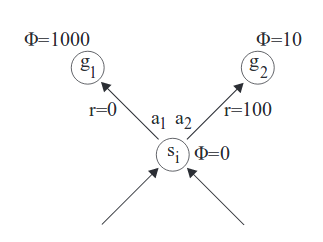
\includegraphics[width=.5\linewidth]{images/reward-shaping-terminal-state}
	\caption{An example that shows why the potential function over terminal state must be 0.}\label{fig:reward-shaping-terminal-state}
\end{figure}

More formally, consider the return of the sequence $\bar{s}$, similarly as Equation \ref{def:expected-discounted-return}:
\begin{equation}\label{def:expected-discounted-return-finite-seq}
\ExpRet(\bar{s}) \defeq \sum_{k=0}^{N-1} \DiscFact^{k}\Reward(s_k, s_{k+1})
\end{equation}

If we apply PBRS, it becomes:
\begin{align}
	\ExpRet_{\Phi}(\bar{s}) &= \sum_{k=0}^{N-1} \DiscFact^{k} (\Reward(s_k, s_{k+1}) + F(s_k, s_{k+1})) \nonumber \\
	&= \sum_{k=0}^{N-1} \DiscFact^{k} (\Reward(s_k, s_{k+1}) + \DiscFact\Phi(s_{k+1}) - \Phi(s_k) ) \nonumber \\
	&= \sum_{k=0}^{N-1} \DiscFact^{k} \Reward(s_k, s_{k+1}) + \sum_{k=1}^{N} \DiscFact^{k}\Phi(s_{k}) - \sum_{k=0}^{N-1} \DiscFact^k\Phi(s_k) \nonumber \\
	&= G(\bar{s}) + \sum_{k=1}^{N-1} \DiscFact^{k}\Phi(s_{k}) + \DiscFact^N\Phi(s_N) - \sum_{k=1}^{N-1} \DiscFact^k\Phi(s_k) - \Phi(s_0) \nonumber \\
	&= G(\bar{s}) + \DiscFact^N\Phi(s_N) - \Phi(s_0) \label{eq:reward-shaping-episodic-terminal-state}
\end{align}
The term $\Phi(s_0)$ cannot alter the policy since does not depend from any action executed; on the other hand, the term $\DiscFact^N\Phi(s_N)$ depends on actions, since the terminal state depends from the previous transitions, hence this term can modify the optimal policy. This happens whenever $\Phi(s_N)\neq 0$, where $s_N$ is any state in which an episode ends, namely goal states, failure states and states where the episode ends due to the time limit exceeded.

A simple solution to this problem is to require that $\Phi(s_N)=0$ whenever the reinforcement learning trajectory is terminated at state $s_N$. Notice that if in other trajectories the same $s_N$ is visited, $\Phi(s_N)$ might be different from 0. The only requirement is that if $s$ is a terminal state, then $\Phi(s) = 0$.

\medskip
\begin{example}\label{exa:reward-shaping-gridworld}
	Recalling Example \ref{exa:gridworld}, we can apply PBRS by defining a potential function that measures how far the agent is from the goal. As heuristic, we can use the \emph{Manhattan distance} between the current position and the goal state. More formally, considering $s_{34}$ the goal state and $s_{ij}$ the current state, we define:
	\[
	\Phi(s) = - [(3 - i) + (4 - j)]
	\]
	It is easy to see that the nearer the agent to the goal state, the higher the potential function evaluated in the state of the agent. For instance, if the current state is $s_{11}$, $\Phi(s_{11}) = - 5$, whereas in $s_{33}$ (which is nearer to the goal), $\Phi(s_{33}) = -1$. 
	With this definition, transition from $s_{11}$ to $s_{12}$ (which makes the agent closer to the goal) evaluates $F(s_{11}, s_{12}) = \Phi(s_{12}) - \Phi(s_{11}) = - 4 - (- 5) = + 1$, whereas for transition $s_{33}\to s_{32}$ (which makes the agent more distant to the goal), $F(s_{33}, s_{32}) = (- 2) - (- 1) = - 1$. 
	
\end{example}

\medskip
In the following sections, we will take into account the topics just described in designing a reward shaping strategy for our setting.

\section{Off-line Reward shaping over $\automaton_\varphi$}\label{sect:off-line-reward-shaping}
In this part we propose an automatic way to apply reward shaping in the setting presented in Section \ref{sect:rl-for-llf-goals}.
Recall that the state space of $\MDPagent^{new}$ is $Q_1\times \dots Q_m \times \States$, where $Q_i$ is the set of states of $\automaton_{\varphi_i}$, the automaton associated to the \LLf formula $\varphi_i$ (see Section \ref{sect:llf2automata}).

The basic intuition about our approach is that \emph{every step toward the satisfaction of a goal formula $\varphi_i$ should be rewarded}, analogously as it is done in reward shaping for classical goals (see Example \ref{exa:reward-shaping-gridworld}). Hence, for a given temporal specification $\varphi_i$ we should assign to every $q\in Q_i$ a potential function that is, to some extent, inversely proportional to the distance from any final state.

Given a (minimal) automaton $\automaton_{\varphi}$ from a \LLf formula $\varphi$ and its associated reward $r$, Algorithm \ref{alg:static-reward-shaping} shows how the potential function is build from $\automaton_{\varphi}$. This operation is made \emph{off-line}, i.e. before the learning process. Then we associate automatically to the states of the \DFA a potential function $\Phi(q)$ whose value decreases proportionally with the minimum distance between the automaton state $q$ and any accepting state. By construction, potential-based reward shaping with this definition of the potential function gives a positive reward when the agent performs an action leading to a $q'$ that is one step closer to an accepting state, and a negative one in the opposite case. Notice that, by construction, $G(\bar{s}) = G_\Phi(\bar{s})$, where $G_\Phi$ is defined in Equation \ref{eq:reward-shaping-episodic-terminal-state}. Indeed, $\DiscFact^N\Phi(s_N) = 0$ because we take into account the issue explained in Section \ref{sect:PBRS-no-gamma}, and $\Phi(s_0) = 0$ by construction of the Algorithm \ref{alg:static-reward-shaping}.

\begin{algorithm}
	\caption{Off-line Reward Shaping over $\automaton_{\varphi}$}
	\label{alg:static-reward-shaping}
	\begin{algorithmic}[1]
		\State $\mathbf{input}$: (minimal) automaton $\automaton_\varphi$, reward $r$
		\State $\mathbf{output}$: potential function $\Phi: Q\to \Reals$
		
		\State Let $sink$ be the sink state after the completion of $\automaton_{\varphi}$
		\State Let $n_{q_0}$ be minimum number of hops to reach an accepting state from $q_0$ \label{alg-line:q0-distance}
		\For{$q\in Q$}:
			\State Let $n_q$ be minimum number of hops to reach an accepting state from $q$ \label{alg-line:q-distance}
			
			\If{$n_{q_0} \neq 0$} \Comment i.e. if $q_0$ is NOT an accepting state
				\State $\Phi(q) \gets \frac{n_{q_0} - n_q}{n_{q_0}} \cdot r$
			\Else	
				\State $\Phi(q) \gets (n_{q_0} - n_q) \cdot r$
			\EndIf

		\EndFor
		
		\State Let $n_{max}$ the maximum number of hops  to reach an accepting state \label{alg-line:max-distance}
		\State $\Phi(sink) \gets \frac{n_{q_0} - n_{max}}{n_{q_0}} \cdot r \ \mathbf{if}\  n_{q_0}\neq 0 \ \mathbf{else}\  (n_{q_0} - n_{max}) \cdot r$ 
		\State \Return $\Phi$
 	\end{algorithmic}

\end{algorithm}

In the actual implementation of the Algorithm \ref{alg:static-reward-shaping}, $\Phi(q)$ can be computed  by least-fix point over the automaton $\automaton_\varphi$, i.e. starting from the accepting states and then explore the states from the nearest to the farthest ones.

\section{On-The-Fly Reward shaping}\label{sect:on-the-fly-reward-shaping}
Reward shaping can also be used when the \DFAs of the \LTLf /\LDLf formulas are constructed \emph{on-the-fly} \citep{AAAI1817342} so as to avoid to compute the entire automaton off-line. To do so we can rely on dynamic reward shaping (see Section \ref{sect:DPBRS}).
The idea is to build $\automaton_{\varphi}$ progressively while learning. During the learning process, at every step, the value of the fluents $\ell \in \L$ is observed and the successor state $q'$ of the current state $q$ of the \DFA on-the-fly is computed. 
Then, the transition and the new state just observed are added into the built automaton at time $t$, $\automaton_{\varphi, t}$, yielding $\automaton_{\varphi, t'}$. The potential function $\Phi$ for $\automaton_{\varphi, t'}$ is recomputed for the new version of the automaton. In this case, the shaping function takes the following form: 
\begin{equation}
F(q, t, a, q', t') = \Phi(q', t') - \Phi(q, t)
\end{equation}
i.e. the dynamic reward shaping in Equation \ref{eq:DPBSF} but taking into account the issue presented in Section \ref{sect:PBRS-no-gamma}
where $\Phi(q, t)$ is a variant of the off-line case, but computed on the automaton $\automaton_{\varphi, t}$. In the following we explain how $\Phi$ in the on-the-fly case differs from the one shown in Section \ref{sect:off-line-reward-shaping}.

\subsubsection{Details about $\Phi(q, t)$}
There is an important issue which has not yet been pointed out. In the \emph{off-line} variant described in Section \ref{sect:off-line-reward-shaping}, we apply reward shaping at every transition by knowing the full automaton $\automaton_\varphi$; however, in the \emph{on-the-fly variant}, at the beginning of the learning task we have an "empty" automaton, i.e. only the initial state with no transition from it. 
Let assume that after an action the automaton makes a move from the initial state. How can we assign a positive/negative shaping reward on the transition if we do not know the goodness of the transition?
And if during a simulation we discover an accepting state, there could be a nearer accepting state that has not yet been discovered, but in order to reach it we should first discover other intermediate states. How to allow the agent to discover it while not fixing on the only known accepting states?

It is clear that, the farther the learning task goes, the more accurate will be the shaping rewards, because every observed transition of the automaton during the activity of the agent is stored and eventually the entire automaton will be explored. However, some paths ending in an accepting state are not fully explored, so how to encourage the agent, in our setting, to explore those paths?

In order to determine $\Phi(s, t)$ for a given $A_{\varphi, t}$, we consider the same computations of Algorithm \ref{alg:static-reward-shaping} but \emph{considering the leaves (wrt the initial state) of the automaton as accepting state}. In this way, even if a path does not end in an accepting state, its following is still rewarded. It could be \emph{wrongly rewarded}, since the path might lead to a failure state. However, the dynamic reward shaping theory states that until the potential-based condition is preserved, also the optimal and near-optimal solutions are preserved; moreover, eventually, once the final state of the path is discovered, the reward for that path will assume the right values.

The search for the leaves states is done through Depth-First Search, while the computation is the same of the Algorithm \ref{alg:static-reward-shaping}.

\medskip
It is easy to see that:

\begin{theorem}
	Automata-based reward shaping, both in off-line and on-the-fly variants, preserves optimality and near-optimality of the MDP solutions.
\end{theorem}
\begin{proof} For the off-line case, the shaping-reward function $\Phi$ is, by construction, potential based, hence fulfilling the premises of theorems in \citep{Ng:1999:PIU:645528.657613} and \citep{Grzes:2017:RSE:3091125.3091208}.
	Also for the on-the-fly variant, we observe that our construction is compliant with the requirements defined in \citep{Devlin:2012:DPR:2343576.2343638}.
\end{proof}
	\chapter{FLLOAT}

\section{Main features}
 
\section{Package structure}
 
\section{Code examples}
 
\section{License}
 
	\chapter{RLTG}

\section{Main features}
 
\section{Package structure}
 
\section{Code examples}
 
\section{License}
 
	\chapter{Experiments}
look at experiment introduction in Grzes phd thesis
\section{\Breakout}



\begin{figure}[h]
	 \centering
	 \begin{subfigure}[b]{0.3\textwidth}
	 	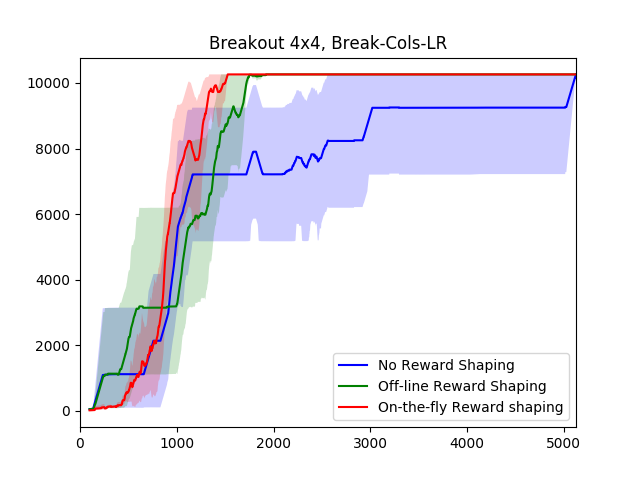
\includegraphics[width=\textwidth]{images/b44-cols-comparison.png}
%	 	\caption{a}
%	 	\label{a}
	 \end{subfigure}
	 ~ %add desired spacing between images, e. g. ~, \quad, \qquad, \hfill etc. 
	 %(or a blank line to force the subfigure onto a new line)
	 \begin{subfigure}[b]{0.3\textwidth}
	 	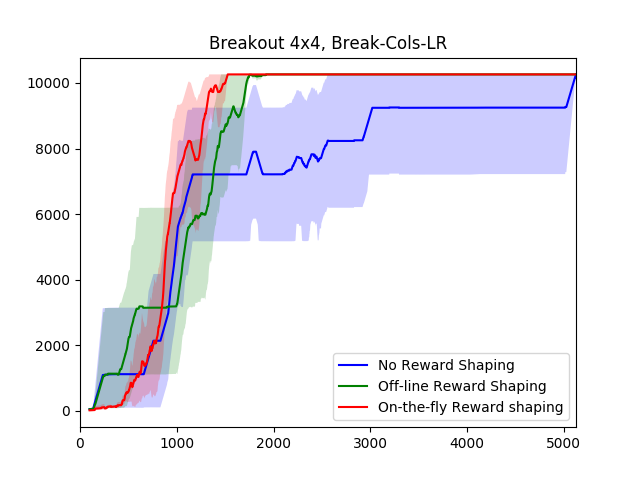
\includegraphics[width=\textwidth]{images/b44-cols-comparison.png}
%	 	\caption{}
%	 	\label{}
	 \end{subfigure}
	 ~ %add desired spacing between images, e. g. ~, \quad, \qquad, \hfill etc. 
	 %(or a blank line to force the subfigure onto a new line)
	 \begin{subfigure}[b]{0.3\textwidth}
	 	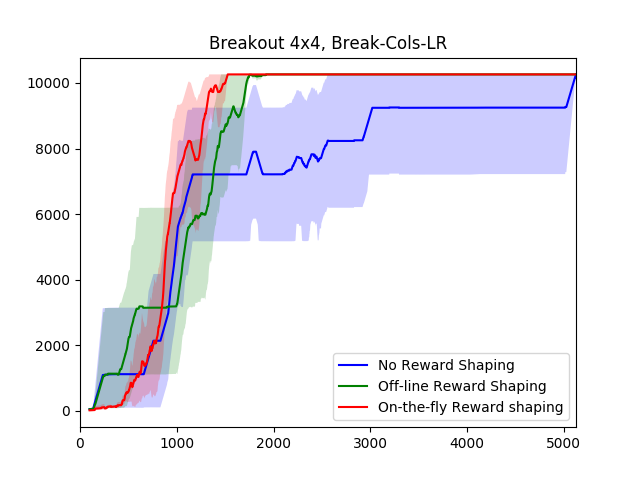
\includegraphics[width=\textwidth]{images/b44-cols-comparison.png}
%	 	\caption{}
%	 	\label{}
	 \end{subfigure}
%	 \caption{}\label{}
\end{figure}

\begin{figure}[h]
	\centering
	\begin{subfigure}[b]{0.3\textwidth}
		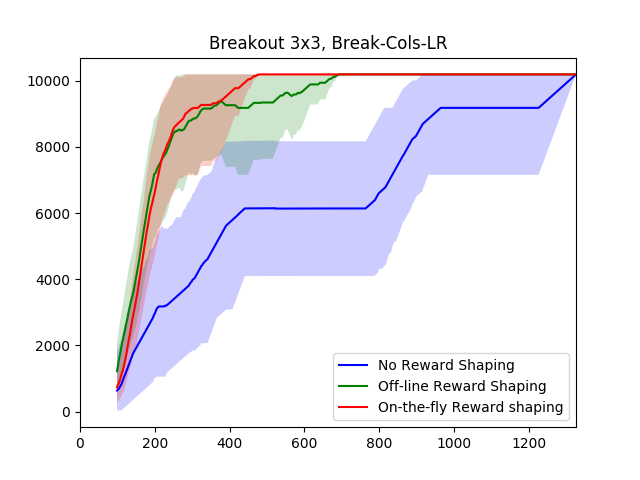
\includegraphics[width=\textwidth]{images/rs-comparison_b33.png}
		%	 	\caption{a}
		%	 	\label{a}
	\end{subfigure}
	~ %add desired spacing between images, e. g. ~, \quad, \qquad, \hfill etc. 
	%(or a blank line to force the subfigure onto a new line)
	\begin{subfigure}[b]{0.3\textwidth}
		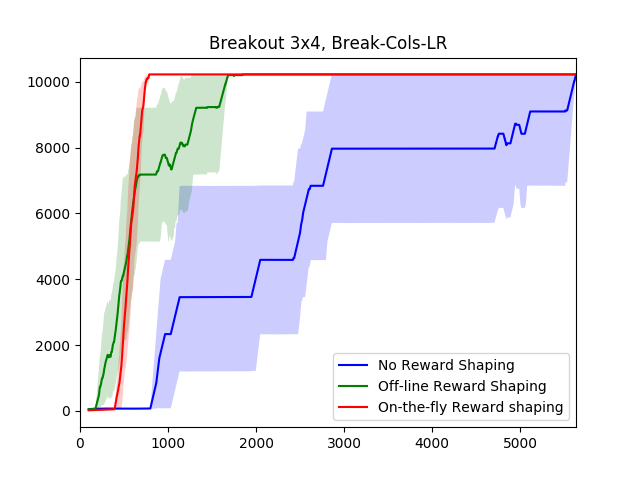
\includegraphics[width=\textwidth]{images/rs-comparison_b34.png}
		%	 	\caption{}
		%	 	\label{}
	\end{subfigure}
	~ %add desired spacing between images, e. g. ~, \quad, \qquad, \hfill etc. 
	%(or a blank line to force the subfigure onto a new line)
	\begin{subfigure}[b]{0.3\textwidth}
		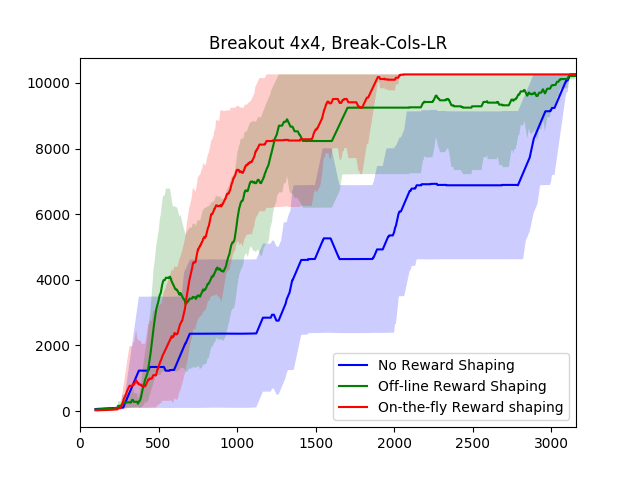
\includegraphics[width=\textwidth]{images/rs-comparison_b44.png}
		%	 	\caption{}
		%	 	\label{}
	\end{subfigure}
	%	 \caption{}\label{}
\end{figure}

\section{\Sapientino}
\section{\Minecraft}
	\chapter{Conclusion and Future Work}\label{ch:conclusions}
This chapter summarizes the thesis. It starts with a brief overview of the problem studied. Then we summarize the main contributions of the thesis. A section is dedicated to future directions of research. The document ends with final remarks.
\section{Overview}
This work addresses a particular problem in reinforcement learning. We considered a classical reinforcement learning problem, i.e. an MDP over a set of features of the world, that we called \emph{low-level} features
\footnote{We say \emph{low-level} features in the sense that these features are only responsible for the basic interaction of the agent with the environment, but still allowing to maximize the reward, or reach the goal in the MDP. Notice that it is only a way to refer about them, and no assumption nor restriction is made over the MDP state space.}.
We are interested in defining non-Markovian rewards over this MDP about some high-level properties of the environment, that we called the \emph{fluents}, determined by some set of \emph{high-level} features of the world.

We considered the cartesian product between the MDP state space and the fluents configurations, which yields, in general, an unknown transition function. 
In order to proceed, we made a key assumption: that is, \emph{the new transition function (i.e. defined both over low-level features and fluents configurations) satisfies the Markov property}, i.e. given the current MDP state, the current fluents configuration and the action taken, we have all the informations needed to know the probability of each state to be the next one.

However, due to the non-Markovian property of the additional rewards, we need to transform the new state space in some way such that the learning is actually feasible and such that the learnt policy in this transformed state space is equivalent (in terms of optimality) to the original problem. How this can be effectively achieved is one of the main contribution of this work.
\section{Summary of Main Contributions}
In this section we list the main contribution of the thesis.
\begin{itemize}
	\item Formal definition and analysis of the problem, as well as design of the transformation of the state space (strongly inspired by \cite{AAAI1817342}), allowing the off-the-shelf reinforcement learning algorithms to actually learn the non-Markovian goals (Chapter \ref{ch:rl}), specified by \LLf formulas (described in Chapter \ref{ch:logic});
	\item An automatic way to apply reward shaping in this setting, leveraging the particular structure of the transformation (Chapter \ref{ch:reward-shaping}). The idea is, the transitions in the new state space that make a step over the automaton towards an accepting state (or, equivalently, any progression in the satisfaction of the formula) should be rewarded. We dealt with both when the automaton is known a priori and when it is built on-the-fly;
	\item Implementation of both the translation algorithm from \LLf formulas to equivalent automata, presented in Chapter \ref{ch:flloat}, and a reinforcement learning framework to set up a RL agent satisfying \LLf formulas, presented in Chapter \ref{ch:rltg};
	\item Experimental evidence that the approach is actually working (Chapter \ref{ch:experiments}).
\end{itemize}

\section{Future Works}
There are many future directions that can be taken, due to the novelty of the work. Some of them are:
\begin{itemize}
	\item the Markov assumption of the combined transition function that has been made in Section \ref{sect:problem-definition} is a strong one; however, in many real world cases, the implicit approximation is not enough to effectively model the world. It might be interesting to find an approach that addresses this issues and manages the problem in this harder scenario.
	\item In this work we prevalently made a theoretical analysis of the problem and we have shown only some application at software level. The proposed framework is more general, and should be validated in many other domains, both simulated and physical ones (e.g. robotics), where there is the need to represent additional high-level knowledge to express complex goals;
	\item We did not focus our attention over the algorithmic side, but only on how the problem can be properly redefined, and relying on off-the-shelf reinforcement learning algorithms. It might be the case that the design of ad-hoc algorithms for this framework yields better performances. For instance, one could think about a better "explicit" exploration policy of the state space, in spite of "implicit" guidance by using reward shaping, and even some adaptation of state-of-the-art techniques, e.g. hierarchical reinforcement learning, curriculum learning, knowledge transfer and so on.
	\item Finally, it could be of interest to extend this work to the general framework of multi-agent systems and work on the challenges and issues that such extension might lead to.
\end{itemize}

\section{Final Remarks}
The topic of this work is of crucial importance: the need to face the dichotomy between the control of low-level features and the ability to reason about higher-level properties of the world is the core issue in many of the fields and applications in artificial intelligence, especially in robotics. This thesis aimed to address this issue in a particular case, by a theoretical analysis, but providing actual implementations as support for the proposed approach.
	
%	\appendix 
%	\chapter{FLLOAT}
%	\chapter{RLTG}

	
	\backmatter
	\phantomsection
	
	\bibliography{bib.bib}
	

\end{document}